\documentclass[12pt,a4paper]{article}
%\usepackage[utf8]{inputenc}
%\usepackage[T1]{fontenc}
\usepackage{xeCJK}
\usepackage{setspace} 
\usepackage{graphicx}

%
\setCJKmainfont{IPAMincho}
\setCJKsansfont{IPAGothic}
\setCJKmonofont{IPAGothic}


\title{私の家族の好きなレストラン\\\small{A Favorite Restaurant of Mine}}
\author{アンドリュー・ローゼン\\ \small{Andrew Rosen}\\\small{JPNS 1001-003}}
\date{}
\begin{document}
	\maketitle
	
	\doublespacing
	
	夏に東京に教えました。
	夏の時、私の家族の好きなレストランはトラットリア・イタリア目黒店でした。
	このレストランはイタリアの食べ物があります。
	
	私の好きなピザはミエールです。
	このピザはチーズとはちみつがあります、でもトマトソースがありません。
	私の子供と私の妻は好きなピザはマルゲリータです。
	すごくおいしです。
	皆さんはやさしいです。
	一次、私は扇子を忘れました。
	おとで、私にこれを返しました。
	
	私と私の家族はそこでよく食べました。
	このレストランはうちの近くでしたから。
	目黒駅の東口を出て、道を綿まて、右へ五分ぐらいです。
	トラットリア・イタリア目黒店は道の左側にあります。
	
	 
	\begin{figure}
		\centering
		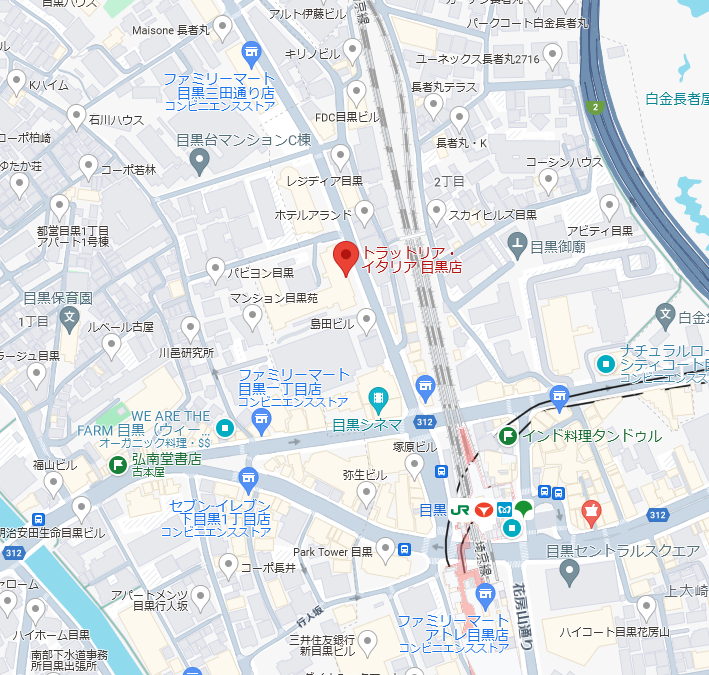
\includegraphics[width=0.7\linewidth]{restaurant}
		\caption{トラットリア・イタリア目黒店}
		\label{fig:restaurant}
	\end{figure}
	

\end{document}